\documentclass{article}
\usepackage[utf8]{inputenc}
%\usepackage{booktabs}
\usepackage{graphicx}
\usepackage{caption}
\usepackage{amsmath}
\usepackage{tikz}
\usetikzlibrary{trees,positioning}
%\usetikzlibrary{positioning}
\newdimen\nodeDist
\nodeDist=20mm
\tikzstyle{arrow} = [thick,->,>=stealth]
\begin{document}
\noindent Ejemplo de Tikz para hacer mapas conceptuales.
\begin{center}
    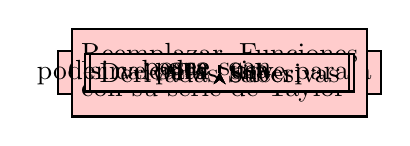
\begin{tikzpicture} [
    node/.style={rectangle,draw,fill=blue!10,rounded corners=.8ex},
    res/.style={thick,rectangle,draw,fill=red!20},
    ]
   
    \node [node] (A) {Serie  de Taylor};
    \path (A) ++(-120:1.2\nodeDist) node [node] (B) {Varias aplicaciones};
    \path (A) ++(-10:2.1\nodeDist) node [node] (C) {Fórmula de Taylor};
    \path (C) ++(-120:\nodeDist) node [node] (D) {Funciones};
				\path (C) ++(-30:1.4\nodeDist) node [res] (E) {Criterios de convergencia};
				\path (B) ++(-145:1.6\nodeDist) node [res] (F) {\parbox[c][2em][c]{4.5em}{Aproximar Funciones}};
    \path (B) ++(-60:\nodeDist)  node [res] (G) {\parbox[c][2.5em][c]{10em}{Reemplazar Funciones con su serie de Taylor}};
    \path (D) ++(-70:\nodeDist)  node [node] (H) {Derivables};
    \path (H) ++(-30:1.5\nodeDist)  node [res] (I) {Cálculo de derivadas};
				\path (H) ++(-120:\nodeDist) node [res] (DS) {Derivadas Sucesivas};
%    \path (G) ++(-120:\nodeDist) node [node] (J) {$D$};
%    \path (G) ++(-60:\nodeDist)  node [res] (K) {0};
%    \path (J) ++(-120:\nodeDist) node [res] (L) {0};
%    \path (J) ++(-60:\nodeDist)  node [res] (M) {1};
   
    \draw[arrow] (A) -- (B) node [left,pos=0.4] {posee}(A);
    \draw[arrow] (A) -- (C) node [right,pos=0.4] {usa}(A);
    \draw[arrow] (C) -- (D) node [left,pos=0.4] {para}(A);
    \draw[arrow] (C) -- (E) node [right,pos=0.4] {usa}(A);
    \draw[arrow] (B) -- (F) node [left,pos=0.4] {sirve para}(A);
	%agregar encontrar la suma y el límite
    \draw[arrow] (B) -- (G) node [right,pos=0.4] {sirve para}(A);
    \draw[arrow] (D) -- (H) node [pos=.5] {que sean}(A);
    \draw[arrow] (H) -- (I) node [right,pos=0.4] {saber}(A);
%    \draw[arrow] (G) -- (J) node [left,pos=0.4] {1}(A);
%    \draw[arrow] (G) -- (K) node [right,pos=0.4] {0}(A);
%    \draw[arrow] (J) -- (L) node [left,pos=0.4] {0}(A);
%    \draw[arrow] (J) -- (M) node [right,pos=0.4] {1}(A);
				\draw[arrow] (H) -- (DS) node [left,pos=0.4] {poder calcular}(A);
    \end{tikzpicture}
\end{center}
\end{document}

